%% LyX 2.2.2 created this file.  For more info, see http://www.lyx.org/.
%% Do not edit unless you really know what you are doing.
%%%%%%%%%%%%%%%%%%%%%%%%%%%%%% User specified LaTeX commands.
%\usepackage{multirow}
%\usepackage{floatrow}

\documentclass[11pt]{article}%
\usepackage[latin9]{inputenc}
\usepackage{amsmath}
\usepackage{amssymb}
\usepackage[authoryear]{natbib}
\usepackage{float}
\usepackage{pdfpages}
\usepackage{graphicx}
\usepackage{amsfonts}
\usepackage{amsthm}
\usepackage{enumerate}
\usepackage{epsfig}
\usepackage{ifthen}
\usepackage{latexsym}
\usepackage{syntonly}
\usepackage{rotating}
\usepackage{lscape}
\usepackage{color}
\usepackage{booktabs}
\usepackage[bottom]{footmisc}
\usepackage{epstopdf}
\usepackage{makeidx}
\usepackage{xr}
% \usepackage{refcheck}%
\setcounter{MaxMatrixCols}{30}
%TCIDATA{OutputFilter=latex2.dll}
%TCIDATA{Version=5.50.0.2960}
%TCIDATA{CSTFile=LaTeX article (bright).cst}
%TCIDATA{LastRevised=Wednesday, August 16, 2023 19:55:35}
%TCIDATA{<META NAME="GraphicsSave" CONTENT="32">}
%TCIDATA{<META NAME="SaveForMode" CONTENT="1">}
%TCIDATA{BibliographyScheme=BibTeX}
%TCIDATA{Language=American English}
%BeginMSIPreambleData
\providecommand{\U}[1]{\protect\rule{.1in}{.1in}}
%EndMSIPreambleData
\textwidth=6.6in
\textheight=8.9in
\headheight=0.0in
\oddsidemargin=0.0in
\headsep=0.0in
\topmargin=0.0in
\newtheorem{theorem}{Theorem}
\newtheorem{corollary}{Corollary}
\newtheorem{case}{Case}
\newtheorem{lemma}{Lemma}
\newtheorem{proposition}{Proposition}
\newtheorem{assumption}{Assumption}
\theoremstyle{definition}
\newtheorem{definition}{Definition}
\newtheorem{example}{Example}
\newtheorem{remark}{Remark}
\def\baselinestretch{1.3}
\newcommand{\abs}[1]{\lvert#1\rvert}
\newcommand{\norm}[1]{\left\lVert#1\right\rVert}
\DeclareMathOperator*{\adjugate}{adj}
\DeclareMathOperator*{\sign}{sgn}
\allowdisplaybreaks
% \externaldocument{Wealth_effect_HARA_Supp_2022}






\begin{document}
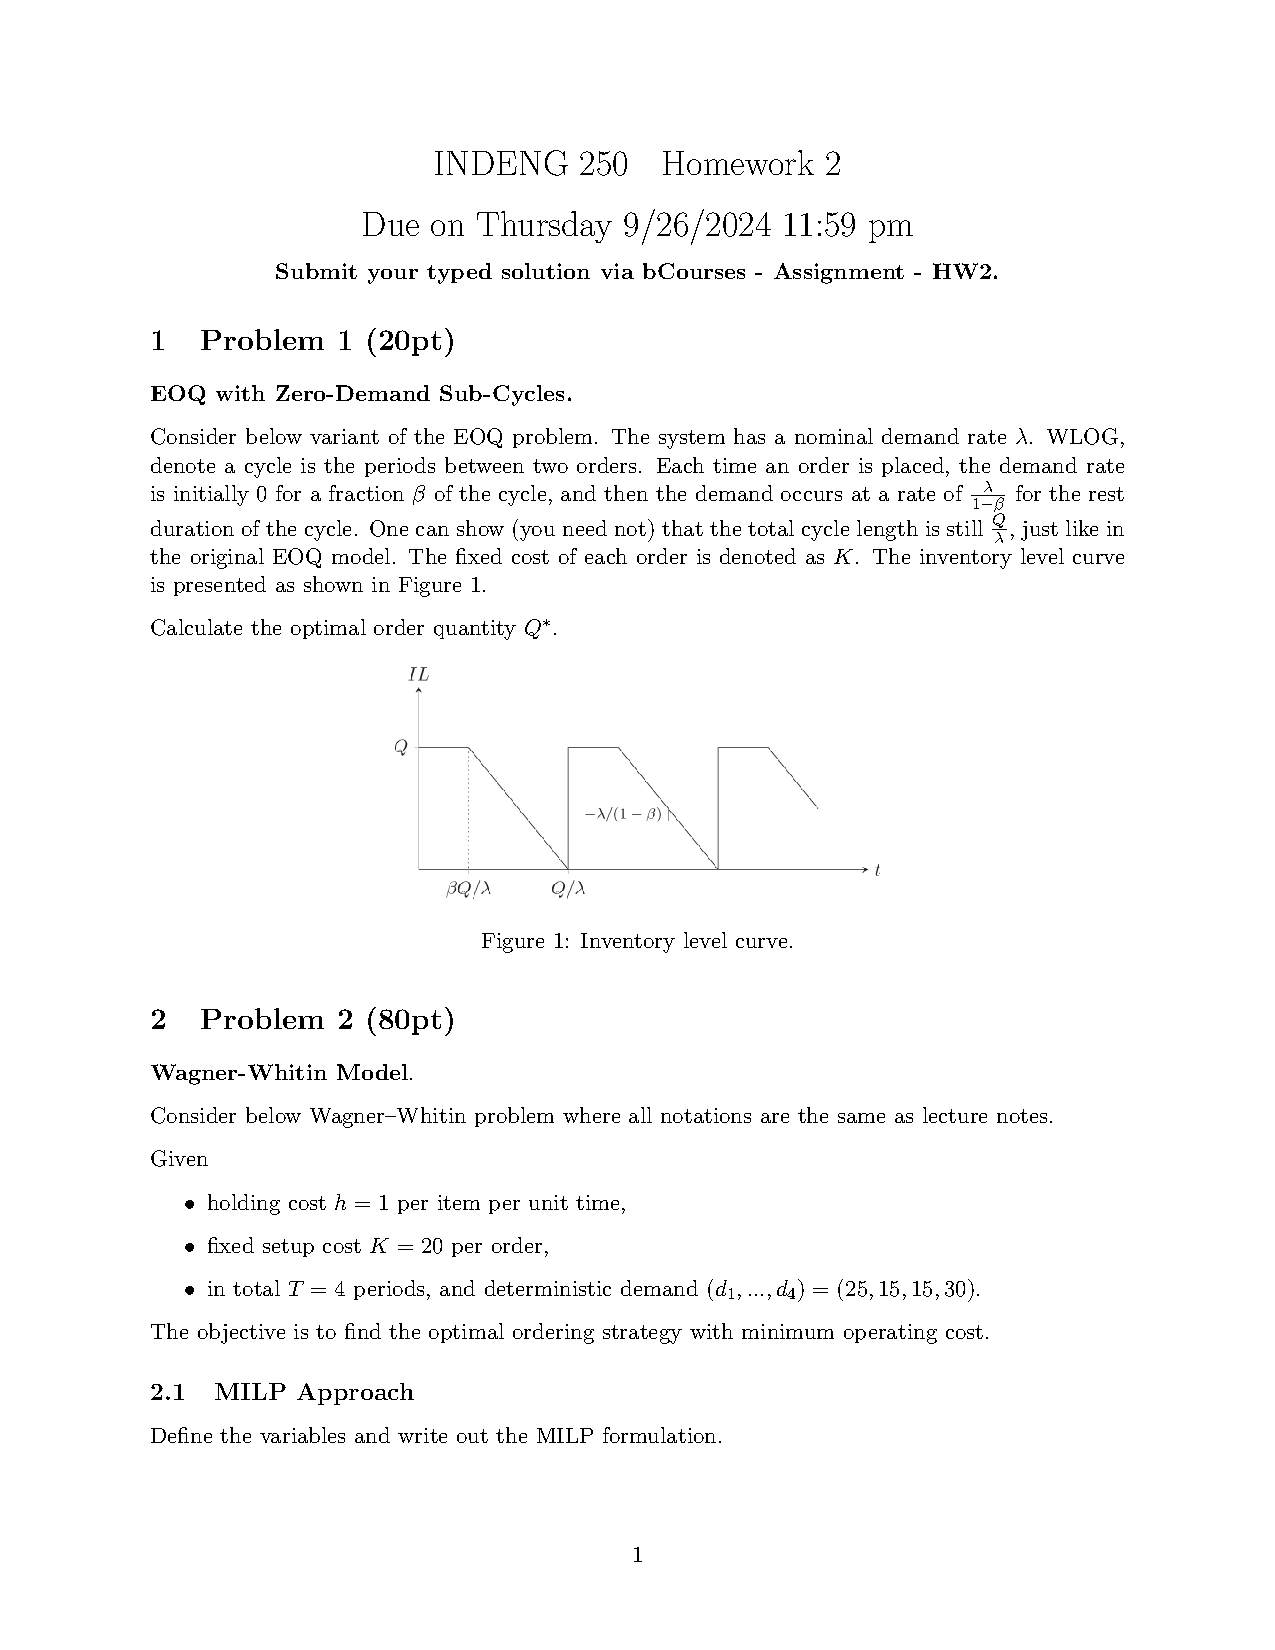
\includepdf[pages={1,2}]{homework_2.pdf}
\title{INDENG 250 PS2}
\author{Junyu Guo}
\date{\today }
\maketitle



1.Now we transform the former EOQ problem into the current problem, we can formulate the cost rate as 
\begin{equation}
    g(Q) =K/(Q/\lambda) + h\left(Q\beta Q/\lambda + (1-\beta)Q/\lambda Q/2\right)/(Q/\lambda),
\end{equation}
we simplify this term and we can have 
\begin{equation}
    g(Q) =\frac{K\lambda}{Q} + h\beta Q + h(1-\beta)Q/2=\frac{K\lambda}{Q} + \frac{(1+\beta)h}{2}Q,
\end{equation}
and we let $g'(Q)=0$, we can have $Q^* = \sqrt{\frac{2K\lambda}{(1+\beta)h}}$.   

2. We first list all the decision variables, we denote
\begin{itemize}
    \item $q_t=$ the number of units ordered in period $t=1,2,3,4$
    \item $y_t=1$ if we order in period $t$, 0 otherwise, $t=1,\cdots, 4$
    \item $x_t$ the inventory level at the end of period, with $x_0\equiv0$
\end{itemize}
We we can list the MILP equations as (with $K=20$ and $h=1$)
\begin{equation}
    \begin{aligned}
        \text{minimize}\quad &\sum_{t=1}^{4} \left(20 y_t+x_t\right).\\
        \text{subject to }\quad &x_t =x_{t-1}+q_t-d_t, \quad\forall t=1,\cdots,4.\\
        &q_t \leq 30y_t, \quad\forall t=1,\cdots,4.\\
        &x_t \geq 0,  \quad\forall t=1,\cdots,4.\\
        &q_t\geq 0,  \quad\forall t=1,\cdots,4.\\
        &y_t\in \{0,1\}, \quad\forall t=1,\cdots,4.
    \end{aligned}
\end{equation}
2.2 Now we attach the results solved by gruobipy. 
\begin{figure}[H]
    \centering
    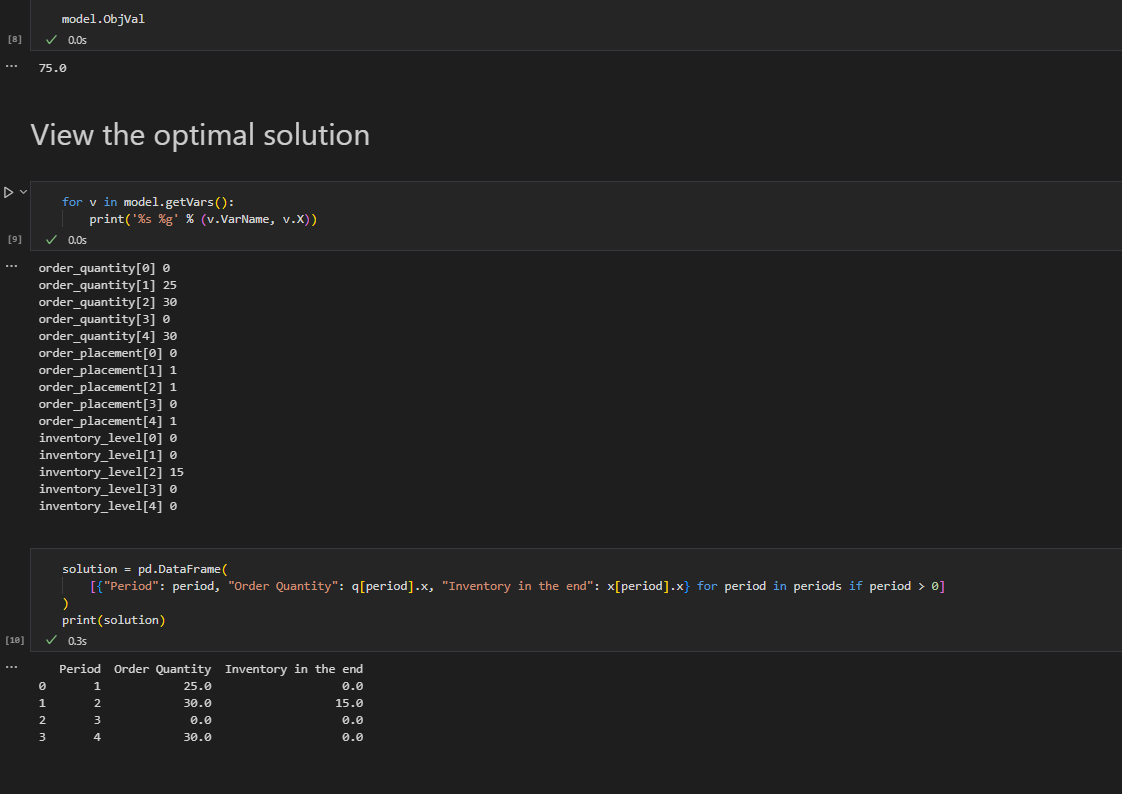
\includegraphics[width=0.9\linewidth]{PS2/code.png}
    \caption{Caption}
    \label{code results}
\end{figure}
We can see that the optimal total cost is 75, and in each period we place an order with quantity 25,30,0,30 respectively. We only place order when $t=1,2,4$.   


2.3 Now we employ the DP approach to solve the same problem.  Now we can derive the recursion with 
\begin{equation}
    \theta_t = \min_{t<s\leq 5} \{20+ \sum_{i=t}^{s-1}(i-t)d_i+\theta_s\}, \theta_5 \equiv 0.
\end{equation}
Using the boundary condition, we can recursively obtain the value for $\theta_t$, $t = 1,\cdots,4$. We have 
    \begin{align*}
        \theta_5 &= 0. \\
        \theta_4 &= 20+0 +\theta_5\\
        &= 20, [s(4)=5].\\
       \theta_3 &=\min\{20+d_4+\theta_5,20+\theta_4\}\\
       &= \min(20+20,20+30) =40, [s(3)=4].\\
       \theta_2 &=\min \{20+\theta_3,20+d_3+\theta_4,20+d_3+2d_4+\theta_5\}\\
       &= \min\{20+40,20+15+20,20+15+60\}=55, [s(2)=4].\\
       \theta_1 &= \min\{20+\theta_2,20+d_2+\theta_3,20+d_2+2d_3+\theta_4,20+d_2+2d_3+3d_4+\theta_5\}\\
       &= \min\{75,20+15+40,20+15+30+40,20+15+30+90\}= 75, [s(1)=2].
    \end{align*}
    The optimal solution goes with 
    order 25 in the first period, and order 30 in the second period, order 0 in the third period and order $d_4=30$ in the last period. 
    The optimal cost should be 180.   

    2.4 Now we use the shortest path algorithm to solve this problem.    \begin{figure}[H]
        \centering
        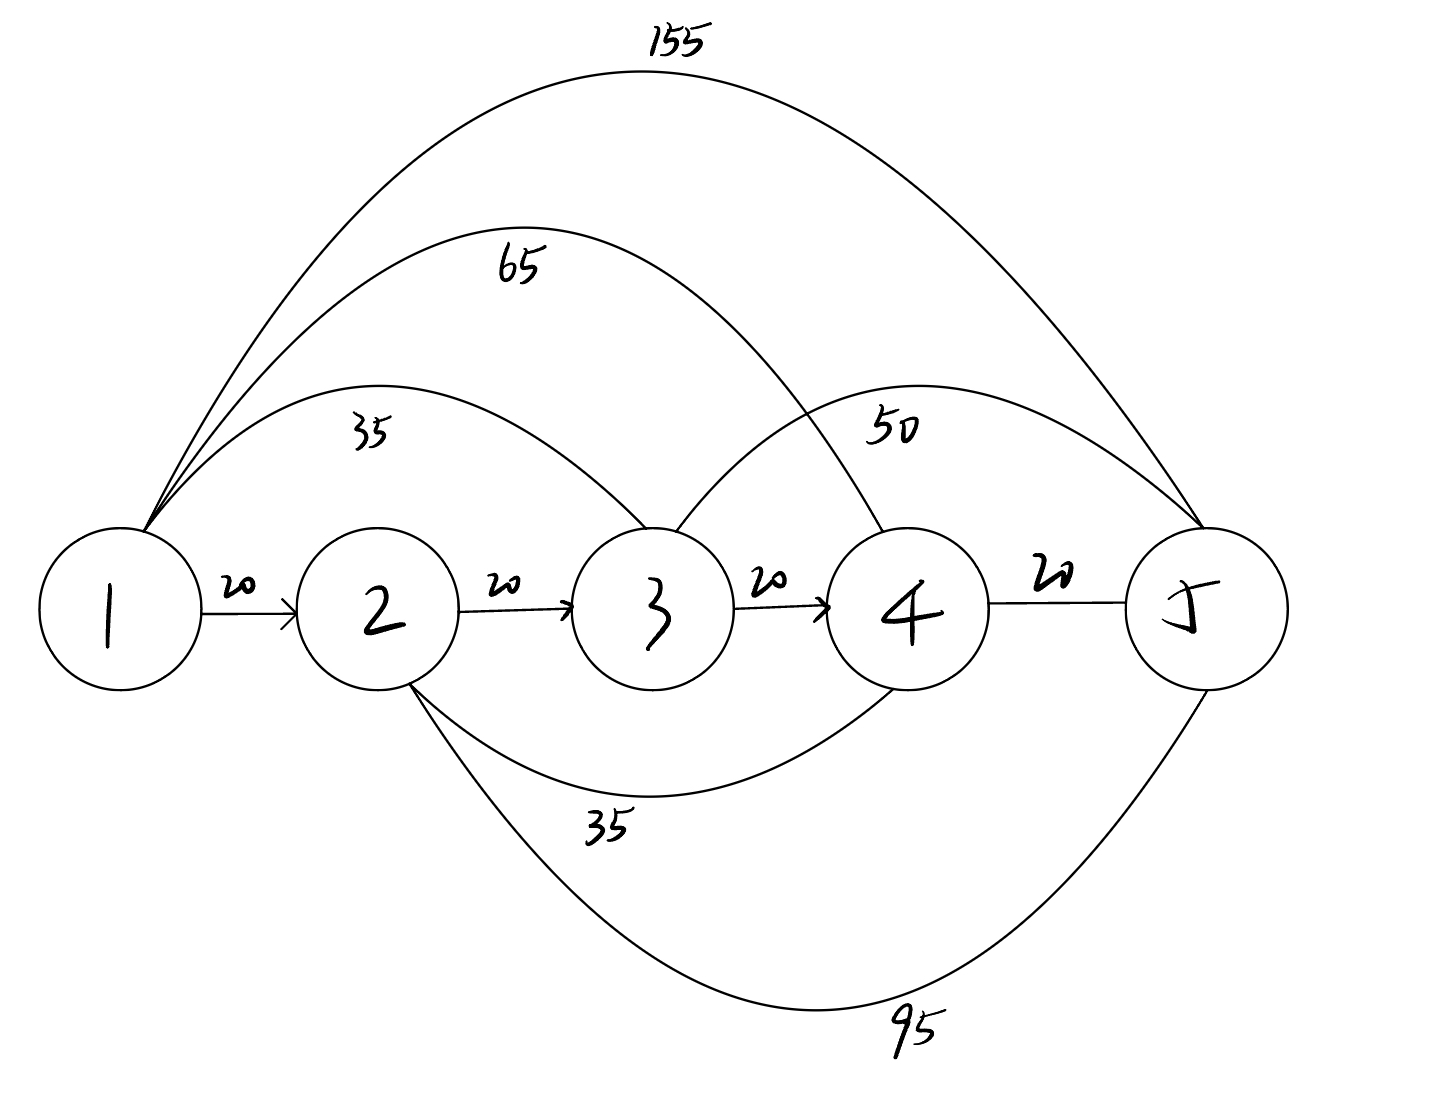
\includegraphics[width=0.5\linewidth]{PS2/graph.jpeg}
        \caption{Graph}
        \label{fig:enter-label}
    \end{figure}
    Now we drive the shortest distance and the shortest path usign the Dijkstra algorithm. 

    In the first round, 
    initialize $X=\{1\}$, $A[1]=0$, $B[1]=\varnothing$. In the first round we can update with 
    \begin{equation*}
        X=\{1,2\}, A[2] =20, B[1] = \{(1,2)\}.
    \end{equation*}
    Now in the second round, we can have that 
    \begin{equation*}
        X=\{1,2,3\}, A[3] =35, B[3] = \{(1,2),(1,3)\}.
    \end{equation*}
    In the second round, we can have that, 
    \begin{equation*}
        X=\{1,2,3,4\}, A[4] =55, B[4] = \{(1,2),(1,3),(2,4)\}.
    \end{equation*}
    Finally in the last round we can have that 
    \begin{equation*}
        X=\{1,2,3,4,5\}, A[5] =20, B[5] = \{(1,2),(1,3),(2,4),(4,5)\}.
    \end{equation*}
    Therefore the optimal path is $1\rightarrow 2\rightarrow 4\rightarrow 5$, in the first round we place the demand at period 1 to fulfill $d_1$, then we directly place an order fulfilling the demand of period 2 and 3 to transition from 2 to 4, which means placing an order of 30 at period 2 and ordering 0 at period 3. Finally, to transition from 4 to 5, we place an order of $d_4=30$. And in this way the optimal cost is 180.
\end{document}